%-------------------------------------------------------------
\section{Modelagem}
%-------------------------------------------------------------
Segundo \citeonline{SOMMERVILLE:2019}, a modelagem de sistemas é definida como ``um processo de desenvolvimento de modelos abstratos de um sistema, cada um apresentando uma visão diferente do mesmo''. Para isso, descreve também que são geralmente usadas notações gráficas baseadas nos tipos de diagrama em \acs{uml} durante o processo de engenharia de requisitos ``para ajudar a derivar os requisitos detalhados de um sistema; durante o processo [...]; e depois da implementação, para documentar a estrutura e operação do sistema'' \cite{SOMMERVILLE:2019}. 

%-------------------------------------------------------------
\subsection{Diagrama de Casos de Uso}
%-------------------------------------------------------------
De acordo com \citeonline{umlGuedes}, o diagrama de casos de uso \acs{uml} é descrito como:

\begin{citacao}
O diagrama de casos de uso [...] tem por objetivo apresentar uma visão externa geral das funcionalidades que o sistema deverá oferecer aos usuários, sem se preocupar com a questão de como tais funcionalidades serão implementadas. [...] É de grande auxílio para a identificação e compreensão dos requisitos do sistema, ajudando a especificar, visualizar e documentar as características, funções e serviços do sistema desejados pelo usuário \cite{umlGuedes}.
\end{citacao}

Logo, a \autoref{diagrama_CasosUso} representa os casos de uso do projeto de sistema \gls{ifriends}.

\begin{figure}[htb]
\centering
\caption{Diagrama de Casos de Uso}
\label{diagrama_CasosUso}
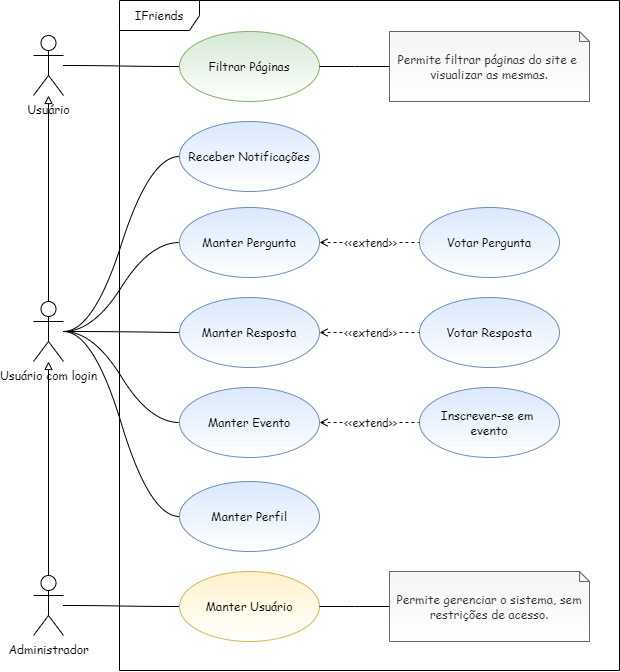
\includegraphics[width=1.0\textwidth]{anexos/Imagens_Diagramas/CasosDeUso_IFriends.png}
\fonte{Os autores.}
\end{figure}
\FloatBarrier

%-------------------------------------------------------------
\subsection{Diagrama de Classes}
%-------------------------------------------------------------
Segundo \citeonline{SOMMERVILLE:2019} os diagramas de classe são usados no desenvolvimento de um sistema orientado a objetos para realizar a demostração das classes e suas associações entre elas. O autor ainda complementa com a seguinte ideia geral: 

\begin{citacao}
De maneira geral, uma classe pode ser encarada como uma definição geral de um tipo de objeto de sistema. Uma associação é um vínculo entre classes, que indica a existência de um relacionamento entre elas. Consequentemente, cada classe pode precisar de alguns conhecimentos a respeito de sua classe associada \cite{SOMMERVILLE:2019}. 
\end{citacao}

Dessa forma, a \autoref{Entidades DdC} representa as entidades do diagrama de Classes do projeto \gls{ifriends}.

% Entidades
\begin{figure}[htb]
\centering
\caption{Diagrama de Classes}
\label{Entidades DdC}
\includesvg[inkscapelatex=false,width=1\textwidth]{anexos/Imagens_Diagramas/Entidades_DiagramaClasses.svg}
\fonte{Os autores.}
\end{figure}
\FloatBarrier

Já a \autoref{Services DdC} representa as classes de serviço e seus respectivos métodos dentro da \gls{api} \gls{ifriends}.

% Services
\begin{figure}[htb]
\centering
\caption{Diagrama de Classes}
\label{Services DdC}
\includesvg[inkscapelatex=false,width=1\textwidth]{anexos/Imagens_Diagramas/Services_DiagramaClasses.svg}
\fonte{Os autores.}
\end{figure}
\FloatBarrier

%-------------------------------------------------------------
\subsection{Diagrama de Entidade e Relacionamento}
%-------------------------------------------------------------
De acordo com \citeonline{leal2015linguagem}, a abordagem entidade-relacionamento é a técnica de modelagem de dados mais difundida e utilizada e representa a modelo conceitual do banco de dados. Nela, a estrutura do banco de dados é descrita como coleção de entidades, relacionamentos e representada graficamente por meio do Diagrama Entidade Relacionamento.

Através dele, é possível descrever um subconjunto do mundo real que será retratado no banco de dados com um alto nível de abstração. Além disso, o modelo Entidade Relacionamento é um modelo formal e caracteriza-se por ter uma grande capacidade semântica, o que garante que todos possam ter o mesmo entendimento \cite{leal2015linguagem}.

A \autoref{diagrama_EntidadeRelacionamento} representa o \ac{der} do projeto de sistema \gls{ifriends}.

\begin{figure}[htb]
\centering
\caption{Diagrama de Entidade e Relacionamento}
\label{diagrama_EntidadeRelacionamento}
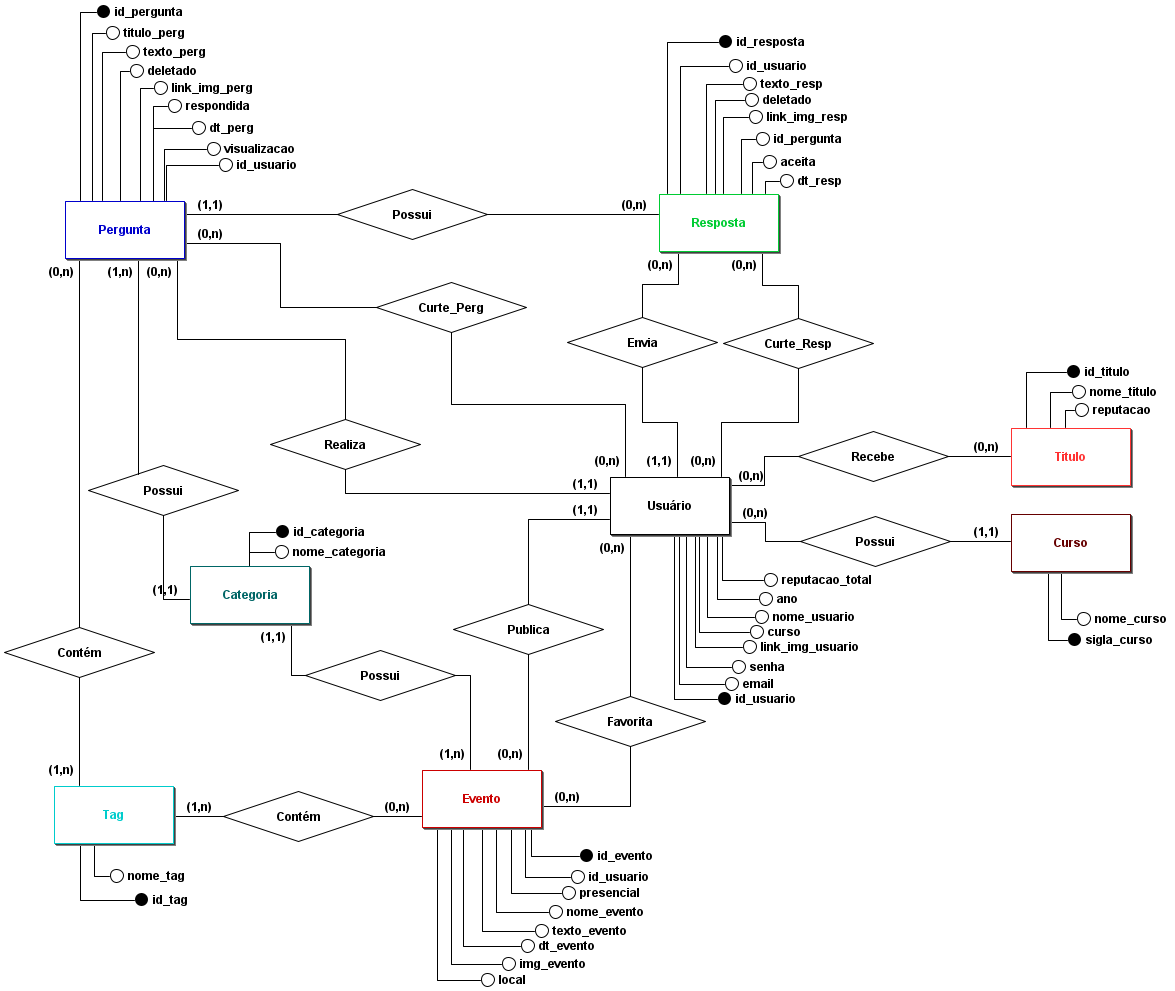
\includegraphics[width=1\textwidth]{anexos/Imagens_Diagramas/DER_IFriends.png}
\fonte{Os autores.}
\end{figure}
\FloatBarrier

%-------------------------------------------------------------
\subsection{Diagrama de Tabelas Relacionais}
%-------------------------------------------------------------
O Diagrama de Tabelas Relacionais \acs{dtr} representa o modelo lógico do Banco de Dados. Segundo \citeonline{utilidadepublica:201?}, através do modelo lógico é representado de maneira mais clara as entidades e os relacionamentos, pois considera algumas limitações e implementa recursos como adequação de padrão e nomenclatura, define as chaves primárias e estrangeiras, normalização, integridade referencial, entre outras.

Deste modo, a \autoref{diagrama_TabelasRelacionais} representa o \ac{dtr} do projeto de sistema \gls{ifriends}.

\begin{figure}[htb]
\centering
\caption{Diagrama de Tabelas Relacionais}
\label{diagrama_TabelasRelacionais}
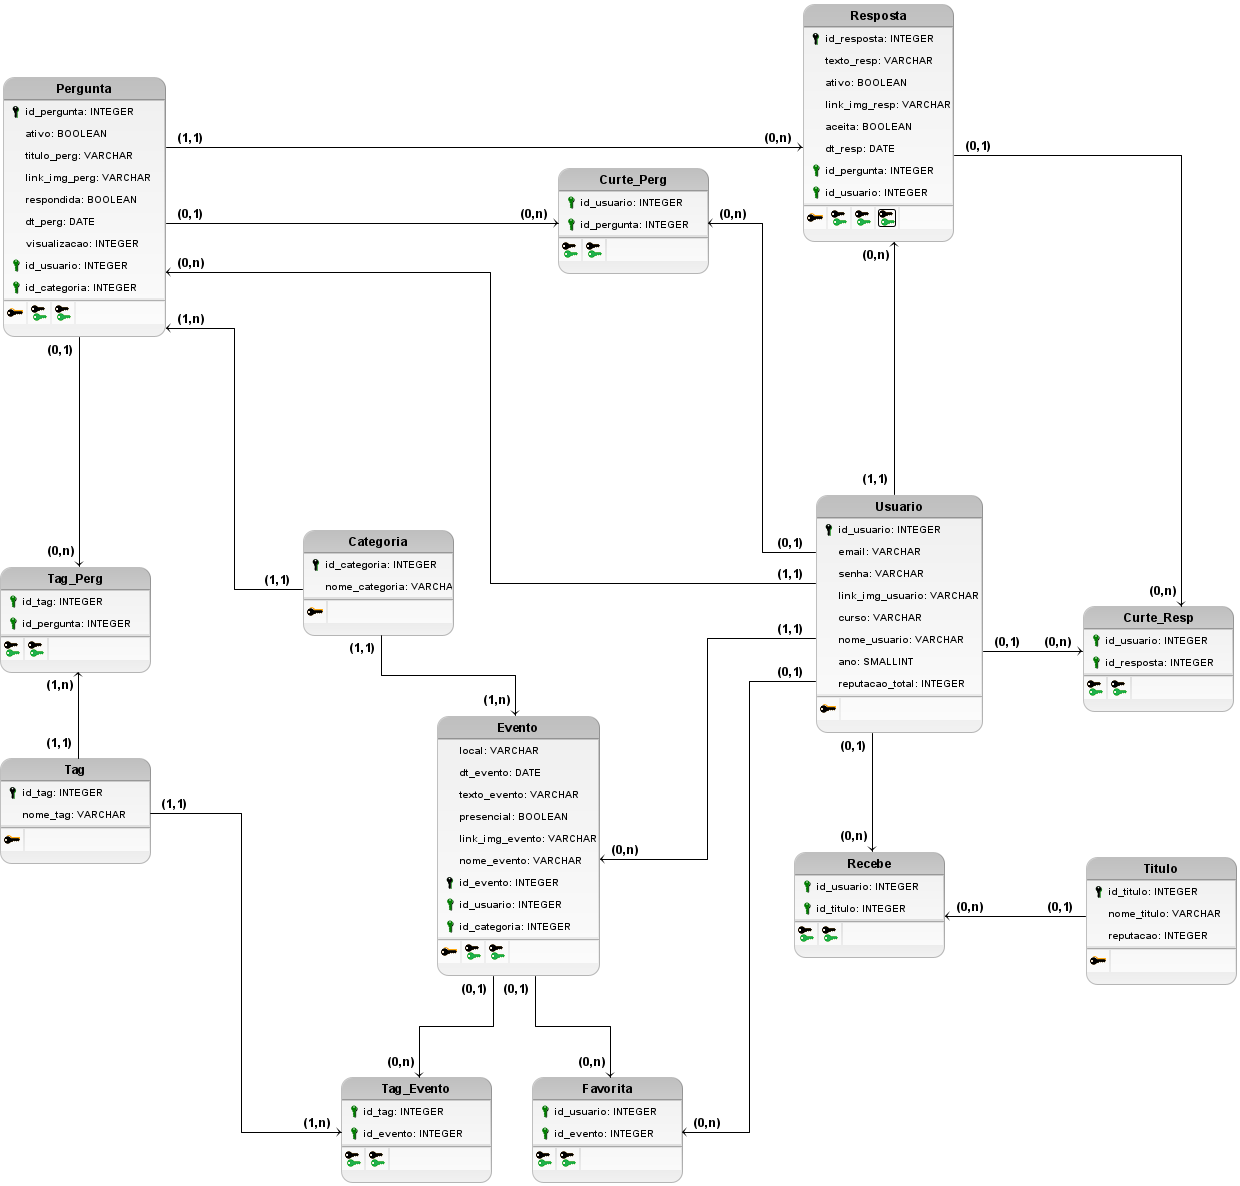
\includegraphics[width=1\textwidth]{anexos/Imagens_Diagramas/DTR_IFriends.png}
\fonte{Os autores.}
\end{figure}
\FloatBarrier

%-------------------------------------------------------------
\subsection{Dicionário de Dados}
%-------------------------------------------------------------
O \ac{dd} é responsável por armazenar as informações de configuração do banco de dados e as estruturas que compõem suas respectivas tabelas. As estruturas definem os campos e suas propriedades \cite{alvesbanco}.

Conforme \citeonline{date2004introdução}, o \ac{dd} é o lugar em que, dentre outras coisas, todos os diversos esquemas (externo, conceitual, interno) e todos os mapeamentos correspondentes são mantidos.

O \ac{dd} contém os metadados, dados que explicam dados, com relação aos diversos objetos que são de interesse do próprio sistema. Exemplos desses objetos incluem índices, usuários, restrições de integridade, restrições de segurança, e assim por diante, informações que essenciais para que o sistema faça seu trabalho apropriadamente \cite{date2004introdução}.

De tal modo, no \autoref{dicionario de dados} encontram-se os quadros que representam o \ac{dd} das tabelas de banco de dados do projeto \gls{ifriends}.
